% !TEX root = ../disertace.tex
%!TEX encoding = UTF-8 Unicode

\chapter{Conclusions and Future work}
\label{sec:conclusion}

\section{Conclusions}

Several years ago, we were thinking about the best way to begin working on improving the state of t-lemmas: to push them a bit forward, from the legacy of surface layer they still carry, towards deeper representation of lexical meaning. Our conclusion was, partly due to our previous experience with annotation using Czech WordNet as the annotation lexicon \citep{holub:2003,bejcek:2006}, was to start by identifying multiword expressions.

We came forward with two hypotheses based on the properties of dependency syntax and specifically of the tectogrammatical description: 1) That each MWE should form a single contiguous dependency structure, and 2) That all instances of a MWE should share the same dependency structure.

After examining a possibility of annotating t-trees directly we came with an idea of an annotation tool that presents a continuous plain text, but links the plain text to the underlying tectogrammatical structure, from which it is generated. 

We proceeded to implement the annotation tool. As an integral part of the tool, we created a system of several types of pre-annotation of data. The most effective pre-annotation is based on the assumptions about tree structures of MWEs. We also devised a simple and efficient way for storing the annotation in a (relatively) human readable and still PML-compliant form by introducing \emph{s-data}. As an important part of the annotation environment, we implemented detailed logs of the annotation that helped us to (at least to some extent) estimate the speed and price of annotation.

We also created a TrEd extension in order to be able to visualise and search s-data together with t-data in TrEd. The extension also provides means to create enriched t-layer that includes MWE annotation. This data can then be used for instance on a PML-TQ server without further dependency on the original s-data.

During our annotation two annotators at a time have annotated multiword expressions and named entities in the whole PDT 2.0 (t-layer). One of the annotators, who was with us for the whole duration of the project, actually annotated about half of the PDT herself.

One of the important result of the annotations is our annotation lexicon \emph{SemLex}: It consists of all the MWEs identified during annotations. All SemLex entries contain tectogrammatical tree structures 

In Section~\ref{sec:annot:pre} we show that the richer and the more consistent the tectogrammatical annotation, the better the possibilities for automatic pre-annotation that minimises human errors. In the analysis of inter-annotator agreement in \Sref{agreement} we show that a weighted measure that accounts for partial agreement as well as estimation of maximal agreement is needed. We present such a measure, deriving it from Cohen's weighted kappa.

The resulting $\kappa_w^U$ has actually been gradually improving (cf. \citealp{biblio:BeStAnnotationMultiword2008}) as we were cleaning up the annotation lexicon, and employing more pre-annotation.

%The methodology of MWE annotation we developed enables precise pre-annotation by automatically extracted tectogrammatical tree structures. We have shown that this pre-annotation should improve annotation speed and should improve also agreement.\footnote{However, we do not present proper statistical tests, so we do not claim, that it does improve the speed and consistency. Only that there are good reasons to believe so.} 

We have shown that the hypotheses about tree structures of MWEs hold, provided the tectogrammatical layer is correctly annotated.\footnote{The only exception (there must always be one, after all) is in the coordinating conjunctions: since our MWE tree structures are built using the ``effective parent'' relation, the coordinating conjunctions are left apart, as they are not the effective parents of their (non-effective) children nodes.} In this respect, our data, especially the places, where different t-structures were (on purpose!) annotated with the same MWE from SemLex, also provide valuable information for both correcting errors and implementing new features in future versions of PDT. 

The annotation tool \code{sem-ann} is freely available under a permissive licence. The annotated data and the annotation lexicon SemLex are also available and will be also published by the Linguistic data consortium. The TrEd extension is available to any TrEd user in the standard extensions repository and is available under the same permissive licence as \code{sem-ann}. For details on availability of tools, data, and licence, see \url{http://ufal.mff.cuni.cz/lexemann/mwe/}.

We believe, however, that we still didn't manage to to properly process all the information that we have acquired during annotation and interesting work still remains to be done.
%
%\section{rozpracovat}
%\xx{Co jsme udelali:} hypoteza o tekto stromech MWE, anotacni nastroj, datovy format pro data, vyuziti hypotezy v predanotaci, \semlex, jeho datova representace, t-stromecky v semlexu, extension -- zobrazeni anotaci a vyhledavani v nich; prvni data, o kterych vime, kde muze i uzivatel hledat shodu a neshodu, apod. (umozneno skvelymi nastroji jinych: PML, tred, pml-tq). Hypoteza potvrzena? Mimochodem anotaci nalezeny chyby v PDT, nektere systematickeho razeni (chybejici uzly v koordinacich?), a take se ukazalo, ze nas blokovaly nedokoncenosti t-lemmat (deminutiva, prechylovani).

%\xx{Zhodnotit vysledky toho, ze nekdy se vyplati anotovat rucne}, a nekdy ne: pripad jmen osob. Zjevne jsme udelali chybu, ze jsme to neanalyzovali takto (viz data od PaSi - EB) drive a nepredanotovali zbytek automaticky podle PDT. Ovsem, nasli by pak anotatori to, co nasli, kdyz by si zvykli na velmi vysokou uspesnost predanotace?
%
%\xx{Pravdepodobnostni pristup k idiomaticnosti} -- mira, nikoliv kategorialni velicina s hodnotami nic, frazem, idiom, ..., ale zaroven mame miru pro mereni vazene shody. 

\section{Future work}
% -- Further analysis of annotation logs
\label{sec:conc:logs}
Considering the price of annotation, it is interesting, how much the annotation process itself stays out of focus of the researchers who create annotated data. Reading the papers and listening to presentations on NLP conferences and the various annotation workshops, one cannot help but see this approach: The data is very interesting, so let us just create it somehow. Almost never is there any published information on the annotation process, factors that influence quality of data, or the price of the results. 

Logs are a  very good source of this valuable information. They can provide an insight into what is actually going on during annotation. Thorough statistical analysis of the logs can provide unbiased information that is hard to get any other way. Better analysis of logs together with s-files can perhaps improve estimation of the real cost of annotation. We have done this during annotation to some extent \see{sec:time-analysis}, but our method is not particularly sophisticated and we just more or less guessed the fluency constant for the annotation intervals.
 
As a small sample of what can be done with the data, we present some further information on the time aspect of annotation work. We decided to have a look at the distribution of times between two consecutive annotation actions\footnote{A helpful suggestion of Zdeněk Žabokrtský.}. We hoped that it can give us more information for properly handling the fluency of annotation intervals discussed in \Sref{sec:time-analysis}. 

We leave it to real statisticians to examine the data more carefully, but our impression is that we used needlessly high value of fluency in our initial estimations described in \Sref{sec:time-analysis}. What is however quite striking in the plots in \Fref{fig:hist} and \Fref{fig:hist-detail}, is the similarity of the histograms. Even though they are not normalised to disregard the different amount of data annotated by each person, the distributions point to a remarkable similarity in behaviour of all three annotators. Compare for instance the distribution for the times up to five seconds. We do not have any explanation or even hypotheses for the uniform raise at 1 second\footnote{histograms actually indicate a lower bound of an interval. 2 seconds thus means $\langle1, 2)$, etc.}, drop at 2, raise at three, etc. It seems to be an interesting point to examine, however.

\begin{figure}[htbp]
   \centering
   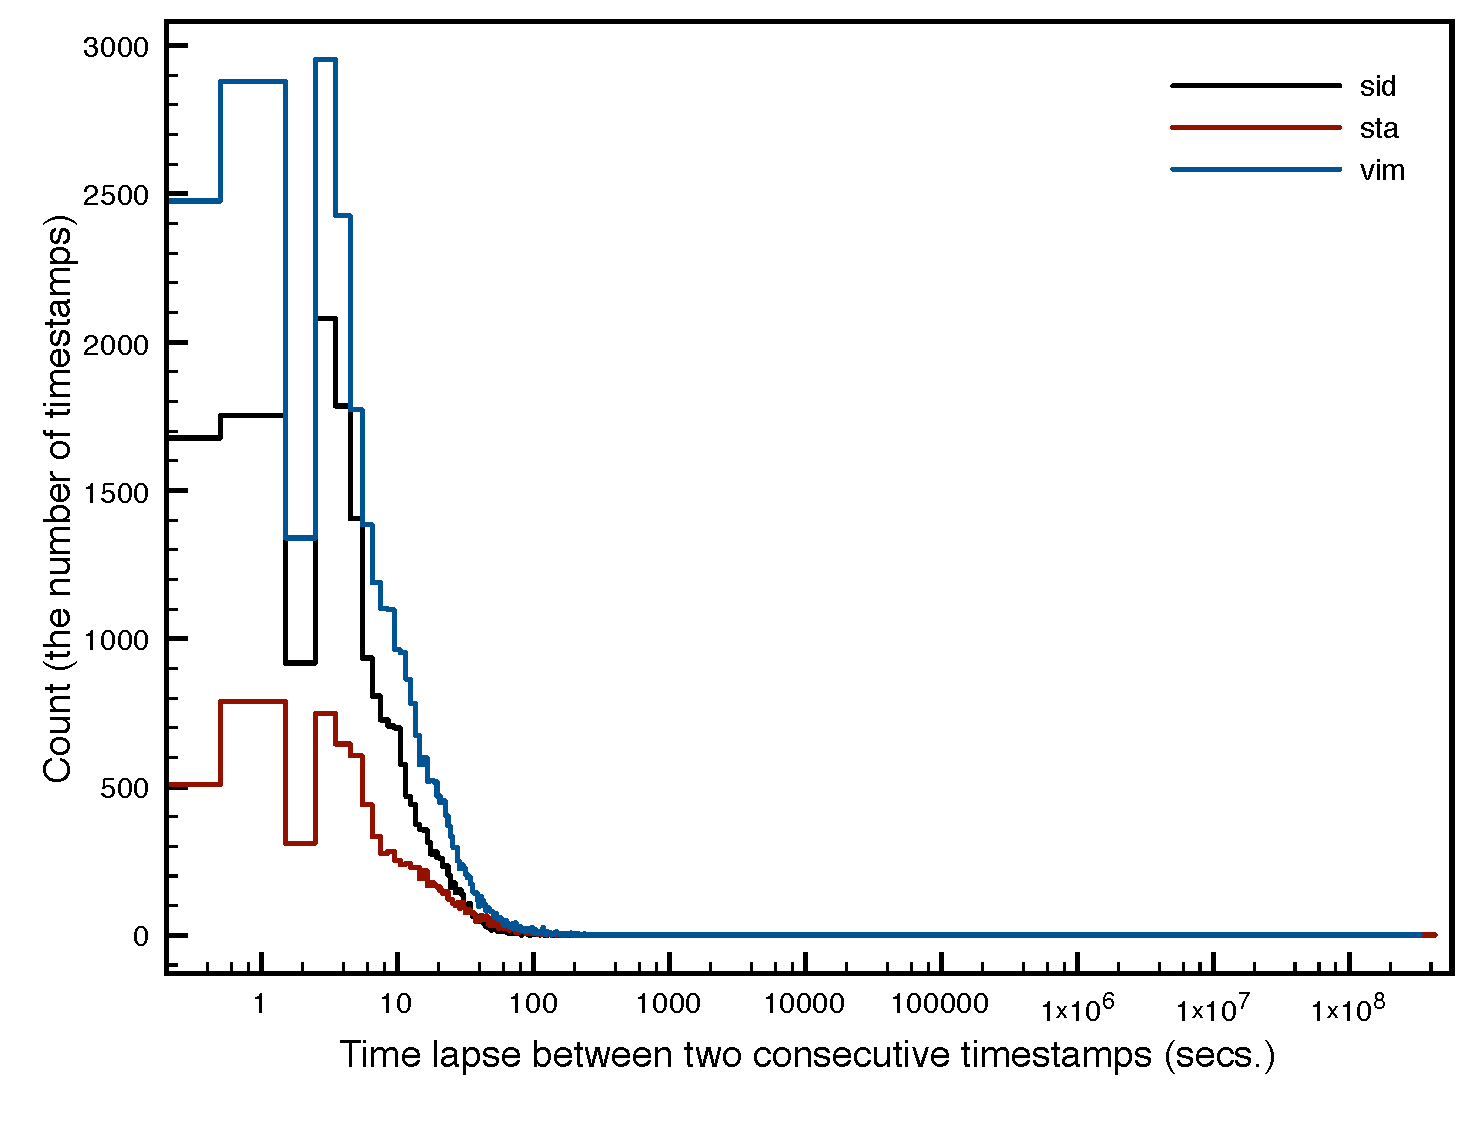
\includegraphics[width=.8\textwidth]{images/speed/histograms} 
   \caption{A histogram showing how many times ($y$) did an annotator place the next tag exactly $x$ seconds after the previous one.} 
   \label{fig:hist}
\end{figure}

\begin{figure}[htbp]
   \centering
   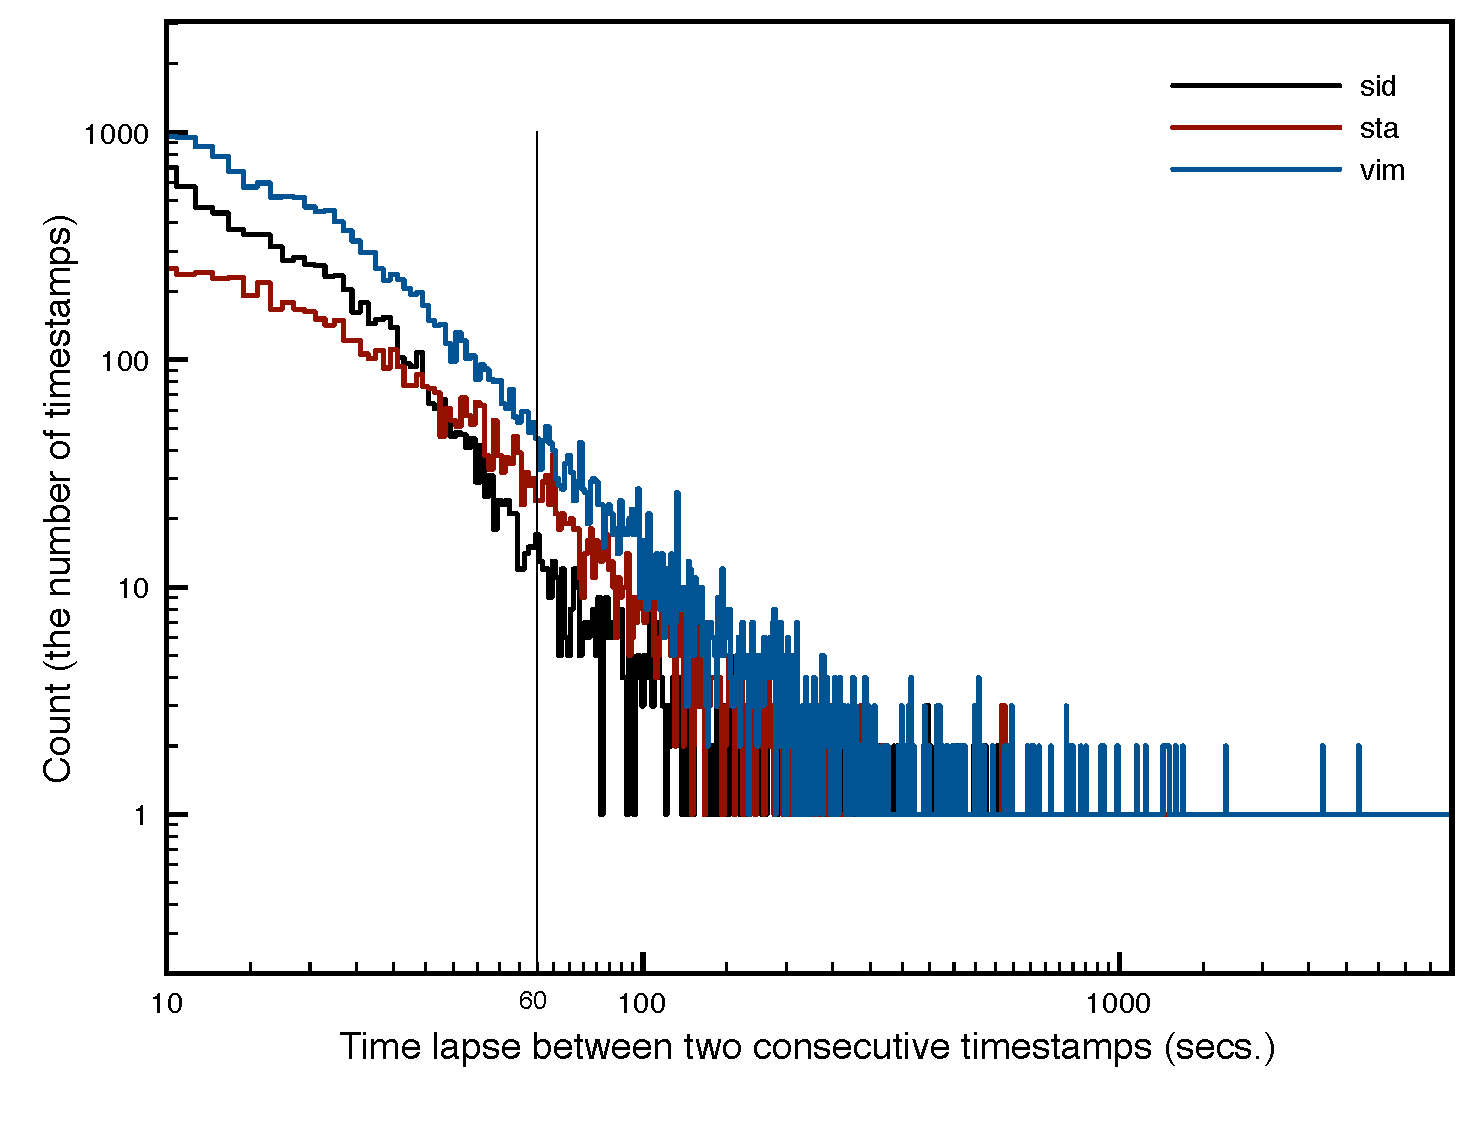
\includegraphics[width=.8\textwidth]{images/speed/histograms-detail} 
   \caption{Detail of the histogram in \Fref{fig:hist} in an interval where we have placed our \emph{fluency} value for the preliminary experiment with clustering of work into annotation intervals ($f=300$, see \Sref{sec:time-analysis} and \Fref{fig:speed}).}
\label{fig:hist-detail}
\end{figure}


But the analysis can go further and, to formulate the problem in economic terms, try to examine in general what factors influence the price of a (correct) tag. What is the relation of speed, length of work intervals, time of day, order of processing of the file, and other factors? We give only a very brief glimpse of one of the factors -- speed of annotation, but in our opinion thorough statistical analysis of log files is an important source of information also for future annotation projects. It may be possible to maximise the efficiency of annotation by experimentally identifying the positive and negative factors. Some of the factors can be quite universal, such as worse concentration after $n$ hours of work, but some may be quite individual (e.g. working in the morning, or on Saturdays\ldots). If some positive and negative factors influencing annotation can indeed be identified, annotation guidelines, both for the project and for the individual annotator can be appropriately modified to maximise the positive and avoid the negative factors.

It is of course possible that in the end no such factors can actually be estimated reliably, at least from our data. But currently we are in a position to seriously examine the possibility and to find out. That is more than has been done until now in any annotation project that we know of. From the little that we can see from our limited experiments, there is already some interesting data that requires interpretation.
